\section{Streszczenie (Executive summary)}
Niniejszy raport stanowi business blueprint projektowanego systemu
klasy ERP dla przedsiębiorstwa zajmującego się produkcją mebli biurowych
oraz świadczeniem usług z nimi związanymi. W raporcie przedstawiono kontekst
biznesowy, modele podstawowych procesów firmy oraz zaproponowano rozwiązanie.
Projekt ma na celu usprawnienie zarządzania
przedsiębiorstwem poprzez integrację procesów biznesowych oraz zapewnienie lepszej
obsługi klienta poprzez efektywniejsze wykorzystanie zasobów.

\section{Kontekst biznesowy}
Przedsiębiorstwo zajmuje się produkcją mebli biurowych,
montażem oraz świadczeniem usług serwisowych. Posiada własny magazyn
oraz wyodrębnioną komórkę zajmującą się sprzedażą.
Firma oferuje system rabatów dla klientów w celu zachęcenia do większych zamówień.
\subsection{Model przedsiębiorstwa}
\begin{center}
    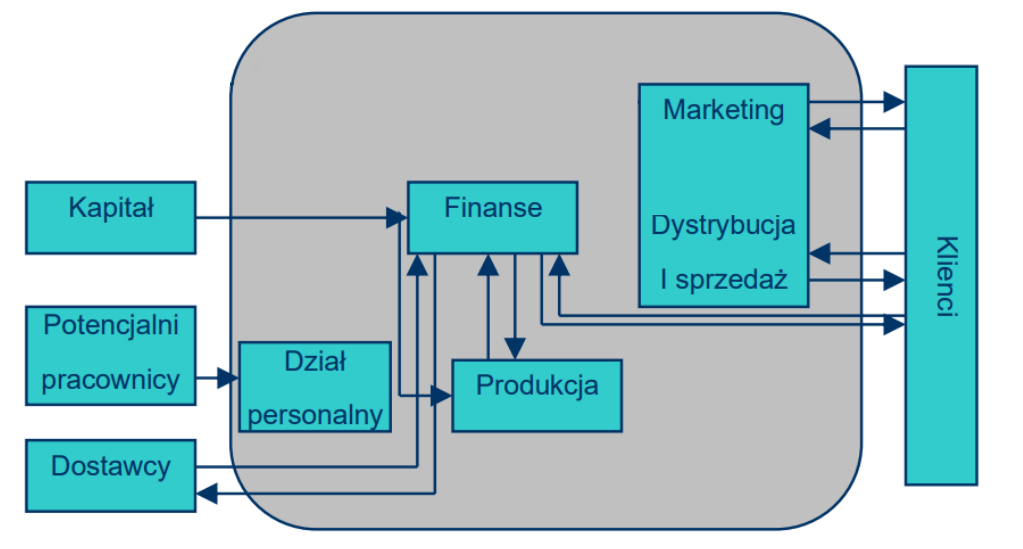
\includegraphics[width=0.9\textwidth]{struktura.png}\\[0.5cm]
\end{center}
\subsection{Struktura organizacyjna}
Firma podzielona jest na działy/ departamenty,
w którym każdy odpowiada za jeden główny cel spójny z jego nazwą,
zgodnie z zasadą divine and conqueor.
\begin{enumerate}
    \item Dział produkcji
    \item Dział sprzedaży i marketingu
    \item Dział obsługi klienta
    \item Dział zasobów ludzkich
    \item Dział logistyki
\end{enumerate}

\section{Modele podstawowych procesów firmy}
\subsection{Proces produkcji mebli biurowych}
\begin{center}
    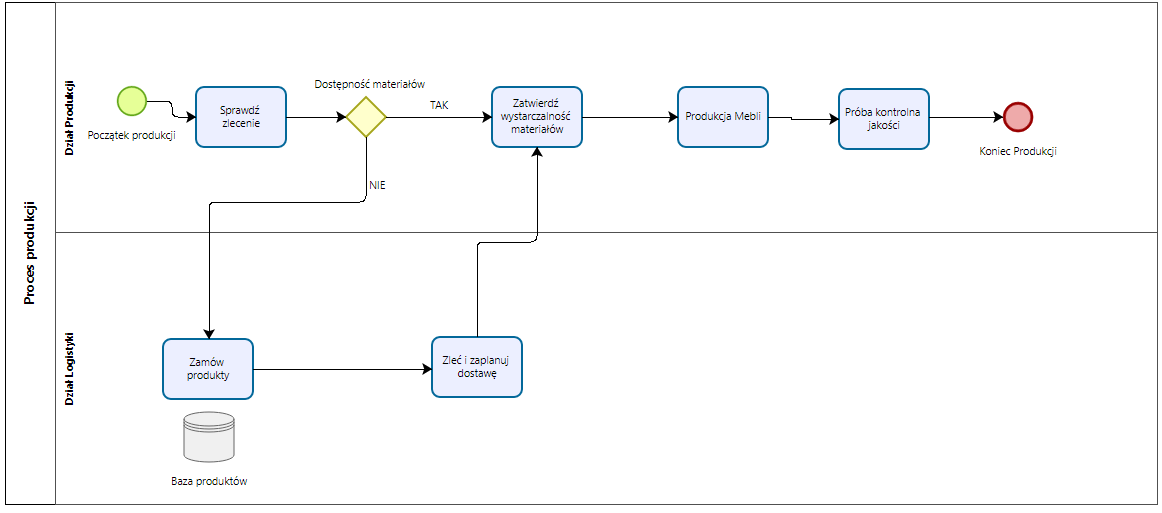
\includegraphics[width=0.9\textwidth]{1.png}\\[0.5cm]
\end{center}
\subsection{Proces montażu}
\begin{center}
    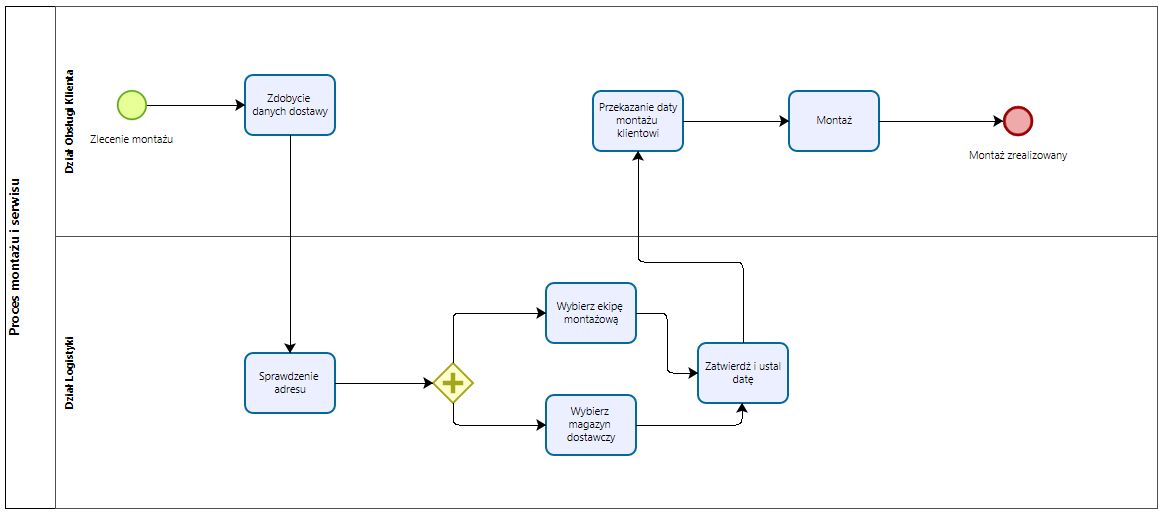
\includegraphics[width=0.9\textwidth]{2.png}\\[0.5cm]
\end{center}
\subsection{Proces zarządzania magazynem}
\begin{center}
    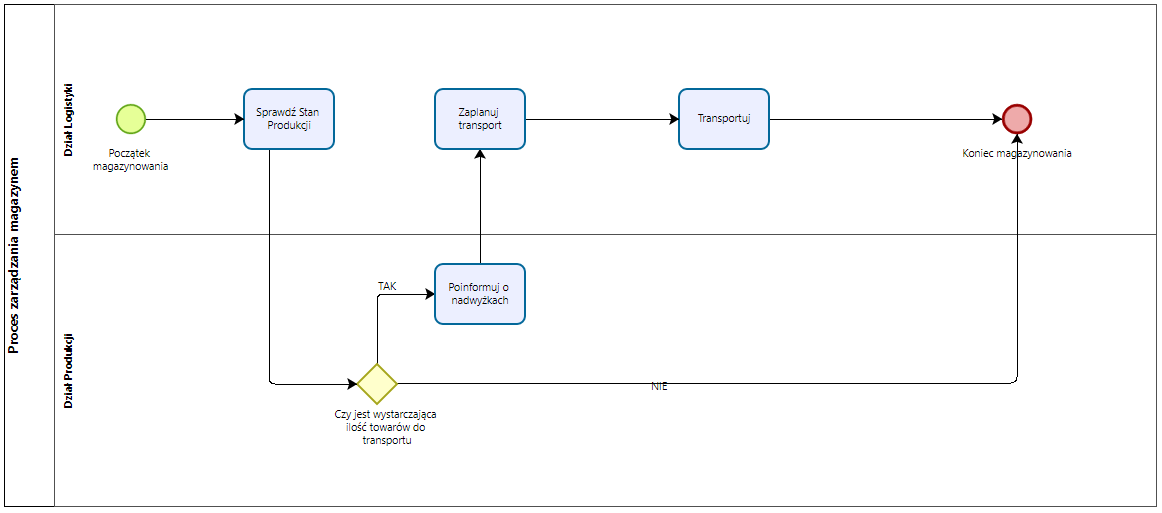
\includegraphics[width=0.9\textwidth]{3.png}\\[0.5cm]
\end{center}
\subsection{Proces sprzedaży}
\begin{center}
    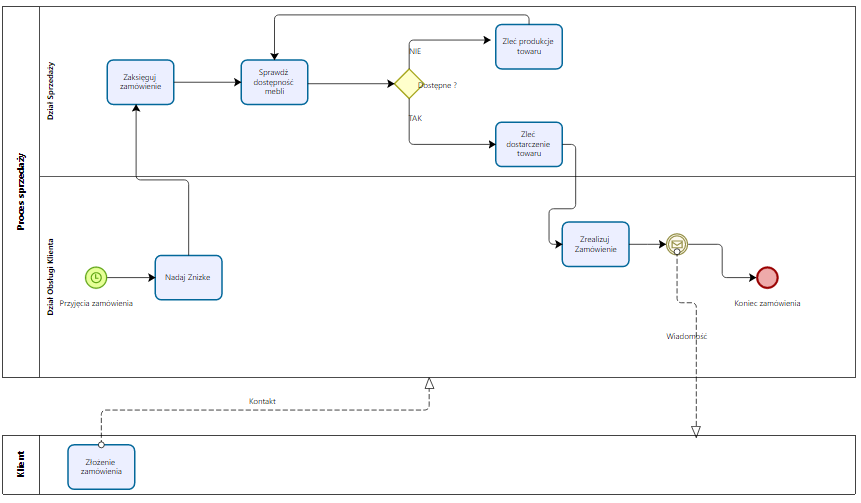
\includegraphics[width=0.9\textwidth]{4.png}\\[0.5cm]
\end{center}

\section{Systemy informatyczne wspierające zarządzanie}
\subsection{Planowanie zasobów przedsiębiorstwa (ERP)}

Planowanie zasobów przedsiębiorstwa (ang. Enterprise Resource Planning – ERP) to zaawansowane systemy informatyczne, które wspierają zarządzanie kluczowymi zasobami i procesami w przedsiębiorstwie. Ich głównym celem jest optymalizacja wykorzystania zasobów, takich jak zasoby ludzkie, materiałowe oraz finansowe, poprzez integrację wszystkich aspektów działalności firmy w jednym spójnym systemie.

Systemy ERP umożliwiają zbieranie, przetwarzanie i analizę danych, co wspomaga podejmowanie decyzji na różnych szczeblach zarządzania. Wspierają zarówno operacyjne, taktyczne, jak i strategiczne zarządzanie przedsiębiorstwem. Dzięki temu firmy mogą efektywnie planować, monitorować i zarządzać swoimi zasobami oraz procesami, co prowadzi do zwiększenia efektywności i konkurencyjności na rynku.

ERP integruje różne funkcje biznesowe, takie jak:
\begin{itemize}
    \item \textbf{Zarządzanie finansami}: Monitorowanie przepływów finansowych, zarządzanie budżetami, księgowością oraz analizą finansową.
    \item \textbf{Zarządzanie zasobami ludzkimi}: Planowanie zatrudnienia, rekrutacja, zarządzanie wynagrodzeniami, szkoleniami oraz rozwojem pracowników.
    \item \textbf{Zarządzanie łańcuchem dostaw}: Planowanie i kontrola zapasów, zarządzanie zakupami, logistyka oraz dystrybucja.
    \item \textbf{Zarządzanie produkcją}: Planowanie produkcji, zarządzanie procesami produkcyjnymi, kontrola jakości oraz optymalizacja produkcji.
    \item \textbf{Sprzedaż i marketing}: Zarządzanie relacjami z klientami, analiza rynku, planowanie sprzedaży oraz kampanie marketingowe.
    \item \textbf{Zarządzanie projektami}: Planowanie, monitorowanie oraz realizacja projektów wewnętrznych i zewnętrznych.
\end{itemize}

Wdrażanie systemów ERP pozwala na automatyzację wielu procesów biznesowych, redukcję kosztów operacyjnych oraz poprawę jakości świadczonych usług. Ponadto, dzięki centralizacji danych, przedsiębiorstwa mogą lepiej koordynować działania pomiędzy różnymi działami, co prowadzi do większej spójności i harmonii w realizacji celów biznesowych.

Współczesne systemy ERP są również skalowalne i elastyczne, co pozwala na ich dostosowanie do specyficznych potrzeb różnych branż i wielkości przedsiębiorstw. Dzięki temu mogą wspierać zarówno małe i średnie firmy, jak i duże korporacje o złożonych strukturach organizacyjnych.

Wdrażanie systemów ERP jest złożonym procesem,
który wymaga starannego planowania i zaangażowania
wszystkich działów przedsiębiorstwa.
Jednak korzyści płynące z ich wdrożenia mogą
znacząco przewyższać początkowe inwestycje,
prowadząc do długoterminowego wzrostu i sukcesu
firmy. Korzyści z wdrożenia systemu ERP to między innymi
\begin{itemize}
    \item \textbf{Zwiększenie efektywności operacyjnej}: Poprawa koordynacji i automatyzacja procesów redukuje czas i zasoby potrzebne do realizacji zadań.
    \item \textbf{Lepsza jakość danych}: Centralizacja danych eliminuje redundancję i zapewnia spójność informacji w całej organizacji.
    \item \textbf{Usprawnienie podejmowania decyzji}: Dostęp do aktualnych i dokładnych danych wspiera analizy i raportowanie, co umożliwia szybkie i trafne decyzje.
    \item \textbf{Optymalizacja kosztów}: Zmniejszenie kosztów operacyjnych poprzez efektywniejsze zarządzanie zasobami i procesami.
    \item \textbf{Zwiększenie elastyczności}: ERP umożliwia szybkie dostosowanie się do zmieniających się warunków rynkowych i wymagań klientów.
\end{itemize}

\section{Optymalizacja Procesu Biznesowego}
\subsection{Model Matematyczny}

W celu minimalizacji kosztów dostawy i montażu dla firmy zajmującej się produkcją i montażem mebli biurowych, definiujemy problem optymalizacji przypisania magazynów do lokalizacji klientów oraz przypisania ekip montażowych. Poniżej przedstawiono matematyczny model tego problemu:

\subsubsection*{Dane wejściowe:}

\begin{itemize}
    \item $M$ - liczba magazynów.
    \item $C$ - liczba klientów.
    \item $cost\_delivery_{ij}$ - koszt dostawy z magazynu $i$ do lokalizacji klienta $j$ (koszt zależny od odległości w kilometrach).
    \item $cost\_installation_{ij}$ - koszt montażu przez ekipę montażową z magazynu $i$ w lokalizacji klienta $j$.
\end{itemize}

\subsubsection*{Zmienna decyzyjna:}

\begin{itemize}
    \item $x_{ij}$ - zmienna binarna, która przyjmuje wartość 1, jeśli magazyn $i$ obsługuje klienta $j$, oraz 0 w przeciwnym razie.
\end{itemize}

\subsubsection*{Funkcja celu:}

Minimalizacja całkowitych kosztów dostawy i montażu:

\[
    \min \sum_{i=1}^{M} \sum_{j=1}^{C} (cost\_delivery_{ij} + cost\_installation_{ij}) \cdot x_{ij}
\]

\subsubsection*{Ograniczenia:}

\begin{enumerate}
    \item Każdy klient musi być obsłużony przez dokładnie jeden magazyn:
          \[
              \sum_{i=1}^{M} x_{ij} = 1 \quad \forall j \in \{1, \ldots, C\}
          \]

    \item Każdy magazyn może obsługiwać co najwyżej jednego klienta:
          \[
              \sum_{j=1}^{C} x_{ij} \leq 1 \quad \forall i \in \{1, \ldots, M\}
          \]
\end{enumerate}

\subsubsection*{Model Matematyczny:}

\[
    \begin{aligned}
         & \min \sum_{i=1}^{M} \sum_{j=1}^{C} (cost\_delivery_{ij} + cost\_installation_{ij}) \cdot x_{ij} \\
         & \text{pod warunkami:}                                                                           \\
         & \sum_{i=1}^{M} x_{ij} = 1 \quad \forall j \in \{1, \ldots, C\}                                  \\
         & \sum_{j=1}^{C} x_{ij} \leq 1 \quad \forall i \in \{1, \ldots, M\}                               \\
         & x_{ij} \in \{0, 1\} \quad \forall i \in \{1, \ldots, M\}, \forall j \in \{1, \ldots, C\}
    \end{aligned}
\]

Ten model matematyczny pozwala na minimalizację kosztów związanych z dostawą i montażem mebli biurowych, uwzględniając odległości między magazynami a lokalizacjami klientów oraz koszty pracy ekip montażowych.
\subsection{Model GNU MathProg}

\begin{tiny}
\begin{verbatim}
# Liczba magazynów i lokalizacji klientów
param M := 3; # liczba magazynów
param C := 3; # liczba klientów

param cost_delivery {1..M, 1..C};
param cost_installation {1..M, 1..C};

# Zmienna decyzyjna: czy magazyn m obsługuje klienta c
var x{1..M, 1..C} binary;

# Funkcja celu: minimalizacja całkowitych kosztów dostawy i montażu
minimize TotalCost: sum{i in 1..M, j in 1..C}(cost_delivery[i,j] + cost_installation[i,j]) * x[i,j];

# Ograniczenia: każdy klient musi być obsłużony przez dokładnie jeden magazyn
s.t. Assign_Clients{j in 1..C}: sum{i in 1..M} x[i,j] = 1;

# Ograniczenia: każdy magazyn może obsługiwać co najwyżej jednego klienta
s.t. Assign_Warehouses{i in 1..M}: sum{j in 1..C} x[i,j] <= 1;

data;
param cost_delivery:
  1 2 3 :=
1 1 2 3
2 4 5 6	
3 7 8 9;

# Koszt montażu przez ekipę z magazynu w lokalizacji klienta
param cost_installation:
  1 2 3 :=
1 10 11 12
2 13 14 15
3 16 17 18;
end;

solve;

# Wyświetlenie wyników
printf "Total Cost: %g\n", TotalCost;
printf "Assignments:\n";
for{i in 1..M, j in 1..C: x[i,j] = 1}{
    printf "Warehouse %d serves Client %d\n", i, j;
}

end;
\end{verbatim}

\end{tiny}

\subsubsection*{Wyniki}

Wyniki skompilowane przez cocoto.github\cite{glpk}.

\begin{center}
    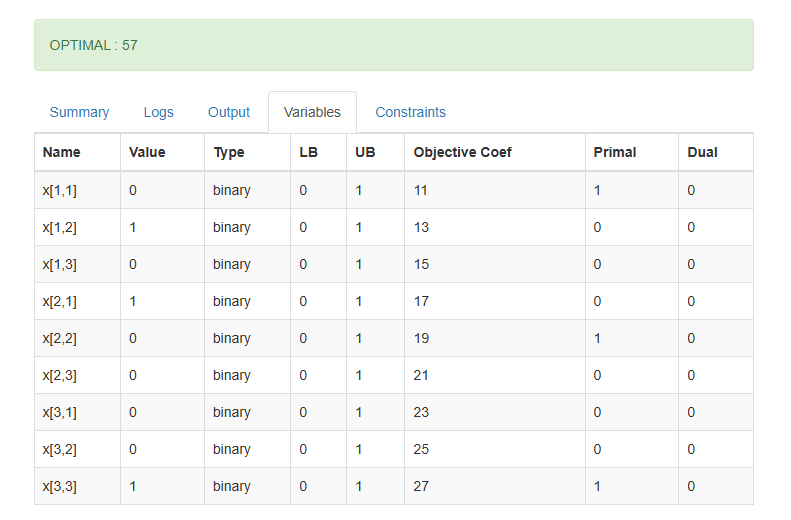
\includegraphics[width=0.9\textwidth]{wyniki.png}\\[0.5cm]
\end{center}

\section{Dane Podstawowe (Master Data)}
Wygenerowany przez PlantUML\cite{plant}.
\subsection*{Diagram Encji}
\begin{center}
    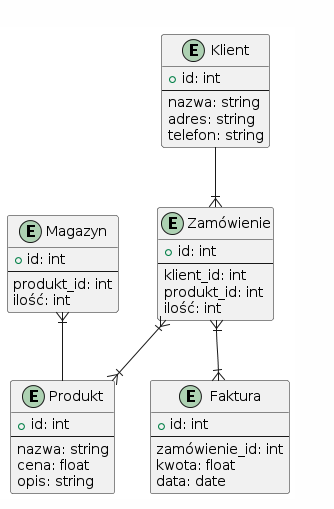
\includegraphics[width=0.6\textwidth]{uml.png}\\[0.5cm]
\end{center}
\subsection*{PlantUML}
\begin{tiny}
    \begin{verbatim}
@startuml
entity "Klient" {
    + id: int
    --
    nazwa: string
    adres: string
    telefon: string
}

entity "Zamówienie" {
    + id: int
    --
    klient_id: int
    produkt_id: int
    ilość: int
}

entity "Produkt" {
    + id: int
    --
    nazwa: string
    cena: float
    opis: string
}

entity "Faktura" {
    + id: int
    --
    zamówienie_id: int
    kwota: float
    data: date
}

entity "Magazyn" {
    + id: int
    --
    produkt_id: int
    ilość: int
}

Klient --|{ Zamówienie
Zamówienie }|--|{ Produkt
Zamówienie }|--|{ Faktura
Magazyn }|-- Produkt

@enduml

\end{verbatim}
\end{tiny}

\section{Strategia wdrażania systemów}

Wykorzystano serwis Odoo \cite{odoo}.

\subsection*{Fakturowanie}
\begin{center}
    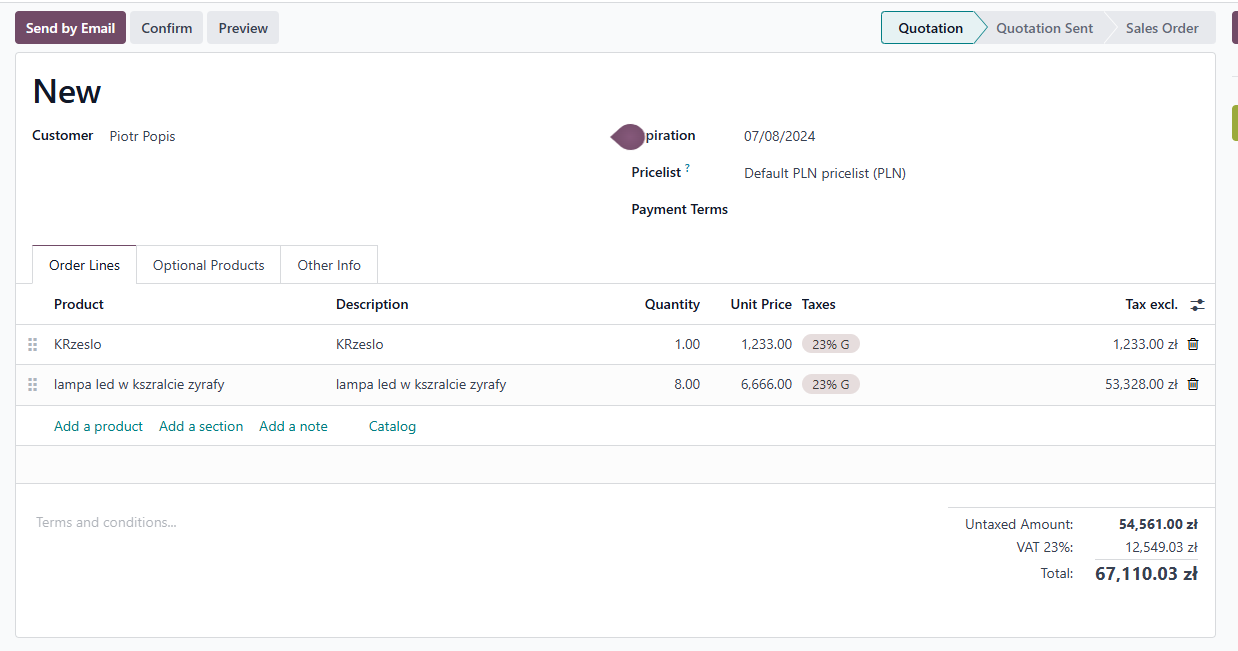
\includegraphics[width=0.9\textwidth]{s1.png}\\[0.5cm]
\end{center}
\begin{center}
    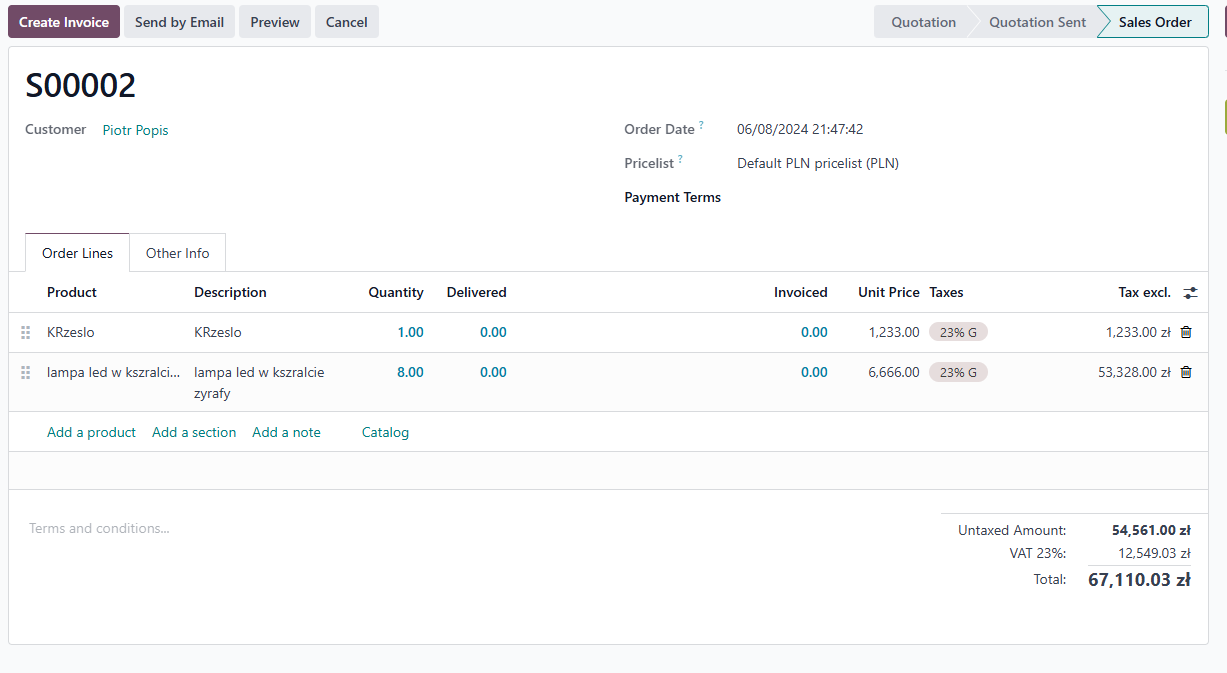
\includegraphics[width=0.9\textwidth]{s2.png}\\[0.5cm]
\end{center}
\begin{center}
    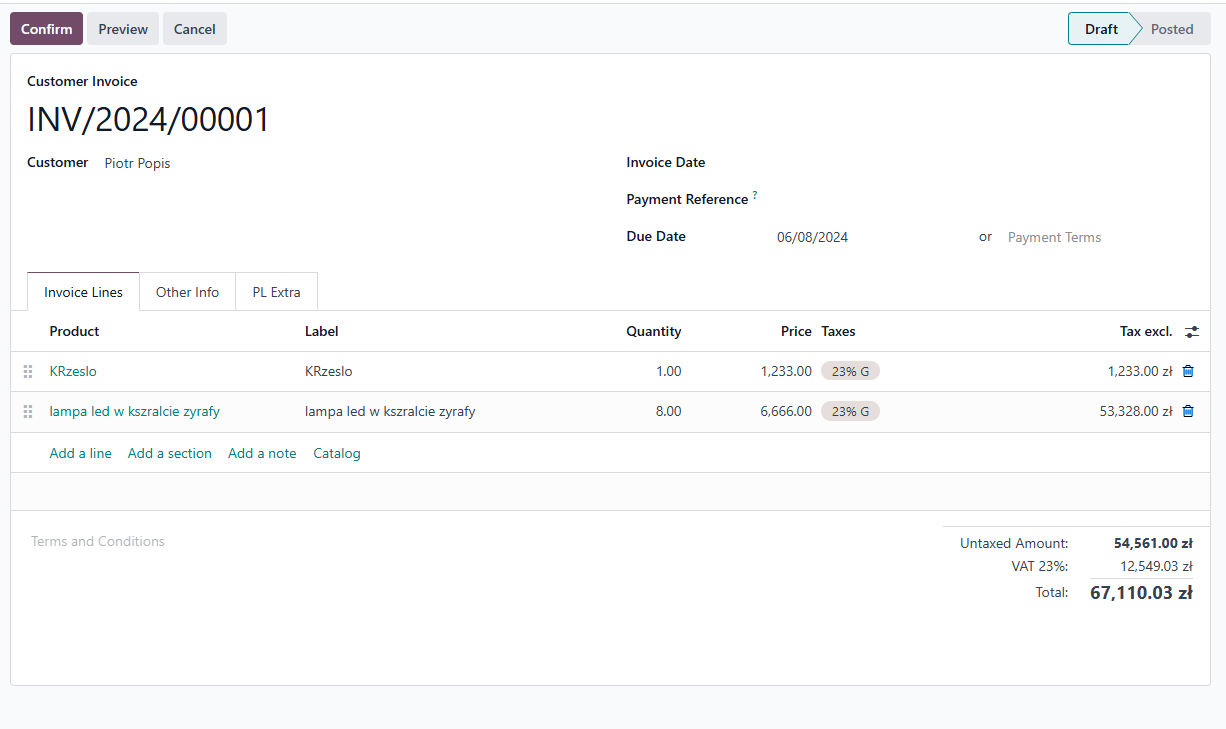
\includegraphics[width=0.9\textwidth]{s3.png}\\[0.5cm]
\end{center}
\begin{center}
    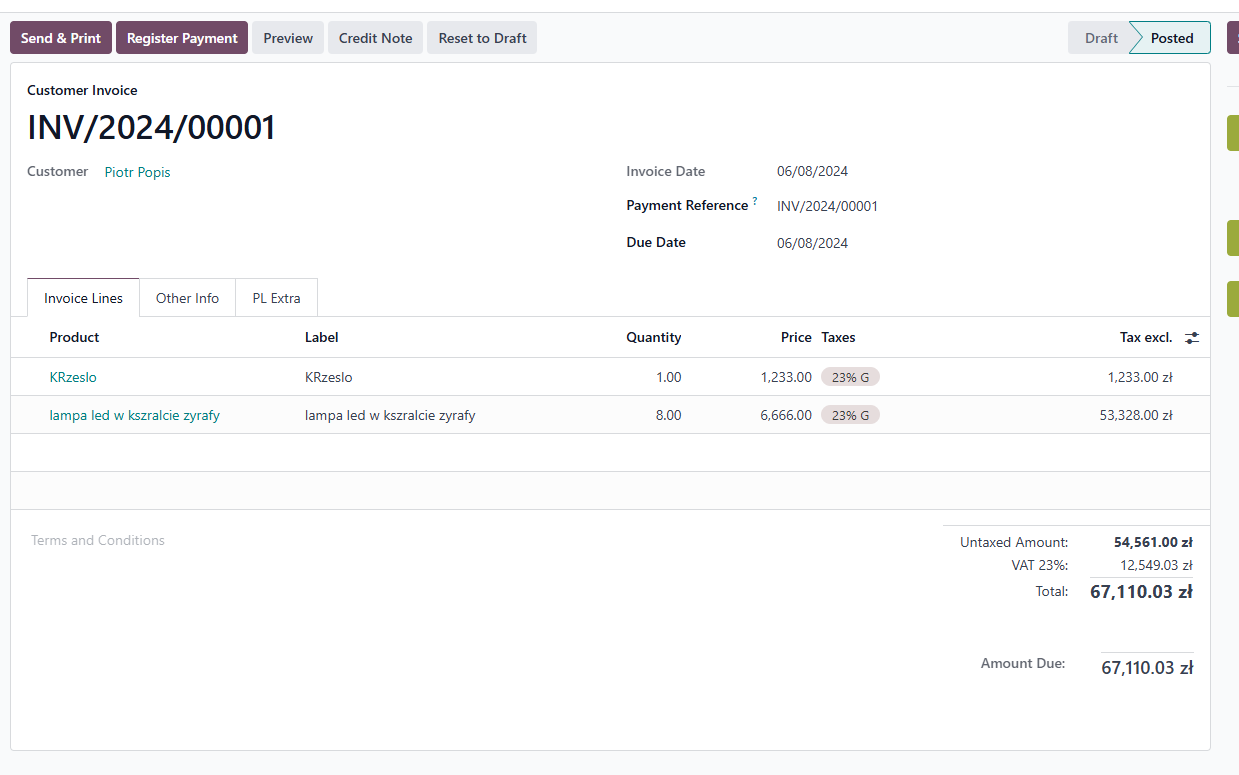
\includegraphics[width=0.9\textwidth]{ss4.png}\\[0.5cm]
\end{center}
\begin{center}
    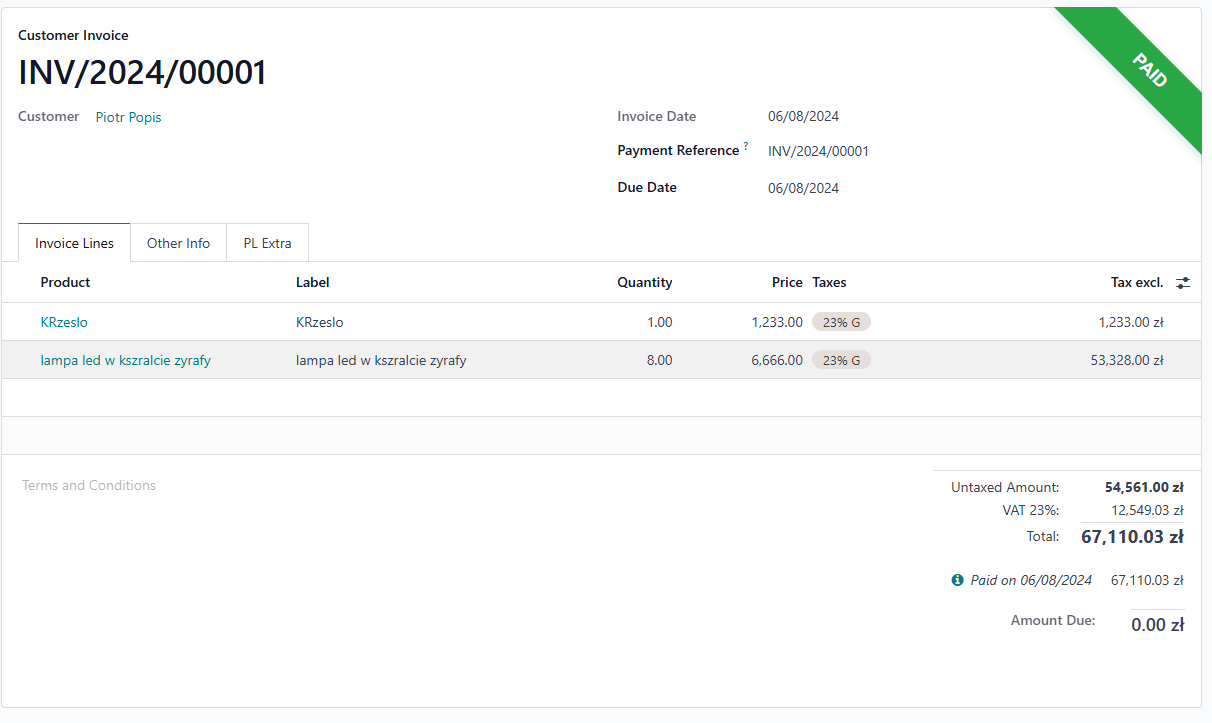
\includegraphics[width=0.9\textwidth]{s5.png}\\[0.5cm]
\end{center}



\subsection*{Magazynowanie}

\begin{center}
    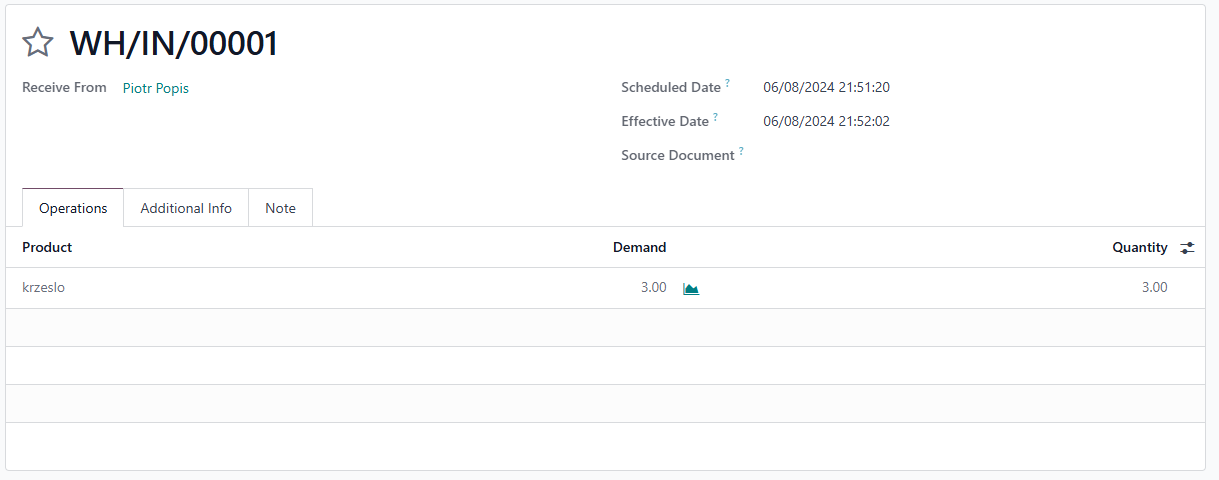
\includegraphics[width=0.9\textwidth]{x1.png}\\[0.5cm]
\end{center}
\begin{center}
    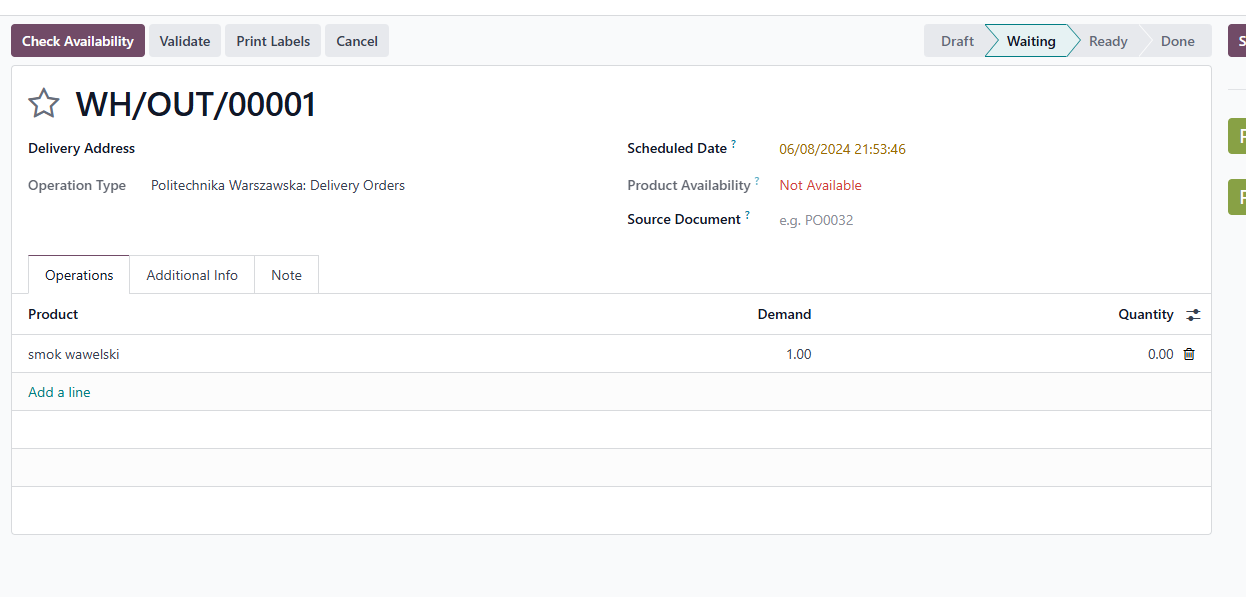
\includegraphics[width=0.9\textwidth]{x2.png}\\[0.5cm]
\end{center}
\begin{center}
    
\includegraphics[width=0.9\textwidth]{x3.png}\\[0.5cm]
\end{center}
\begin{center}
    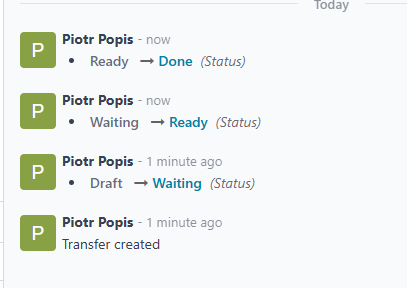
\includegraphics[width=0.9\textwidth]{s4.png}\\[0.5cm]
\end{center}
\begin{center}
    
\includegraphics[width=0.9\textwidth]{x4.png}\\[0.5cm]
\end{center}